\hypertarget{seccion:IniciarSesion}{\vspace{1pt}}
\section{Marco Teórico}

\subsection{Big Data}
El término Big Data se refiere a cantidades enormes de información, por ejemplo, la cantidad de información que se produce todos los días con el uso de una red social como Facebook, o la cantidad de datos que producen computadoras y dispositivos electrónicos que se auto monitorean mediante sensores. Esos volúmenes masivos de datos pueden ser utilizados para extraer conocimiento de ellos, y posteriormente atacar problemas que no sería posible resolver sin el Big Data.

\subsubsection{Las 3 Vs del Big Data}
Al ser el Big Data un concepto emergente y relativamente nuevo, se han tenido ciertas dificultades para definirlo de manera uniforme. Debido a las dimensiones de todo lo que conlleva entender Big Data, resultó conveniente entre los estudiosos del tema definir y acentuar las magnitudes que lo definen. Estas magnitudes se conocen como las 3 Vs del Big Data.

\begin{enumerate}
	\item \textbf{Volumen:} Con Big Data, se tendrán que procesar enormes volúmenes de información. Este punto es importante ya que el crecimiento de la nececidad de almacenamiento de datos en el mundo moderno, crece de forma exponencial.
	\item \textbf{Velocidad:} Usando Big Data, se abre la posibilidad de acceso y flujo de datos a velocidades que no se podrían conseguir de manera convencional.
	\item \textbf{Variedad:} Procesamiento de datos de naturaleza heterogénea, es decir, múltiples tipos de datos.
\end{enumerate}

\subsubsection{Casos de uso del Big Data}

\begin{UClist}
	\UCli \textbf{Desarrollo de productos:} Compañías como Netflix y Procter \& Gamble utilizan el Big Data para anticiparse a la demanda de los consumidores de sus productos. Utilizan modelos predictivos para sus nuevos productos clasificando atributos clave de sus anteriores productos modelando las relaciones entre esos atributos.
	\UCli \textbf{Mantenimiento predictivo:} Se pueden predecir fallas mecánicas en maquinaria que de otra forma quedarían fácilmente ignoradas. Mejorando así ampliamente la calidad y el costo del mantenimiento de dichos equipos.
	\UCli \textbf{Experiencia de usuario:} El uso de Big Data permite recopilar toda la información sobre el usuario y utilizarla a favor de su experiencia en un sitio o aplicación. Por ejemplo, sus búsquedas frecuentes, los sitios que visita, etc. Para de esta manera empezar a hacerle ofertas o anuncios personalizados, según sus intereses particulares.
	\UCli \textbf{Machine Learning:} Actualmente el machine learning es un área de mucho auge, ya que permite entrenar a las computadoras mediante conjuntos de datos de entrenamiento en lugar de programarlas. El Big Data facilita esa tarea.
\end{UClist}

\subsection{Minería de datos}
La minería de datos es el proceso de generar conocimiento a partir de un conjunto de información de gran tamaño. Para generar ese conocimiento se utilizan diferentes técnicas de análisis que detectan patrones y tendencias en la información que se está procesando. Si se intentara utilizar algún método de análisis tradicional, sería muy complicado o incluso imposible a veces encontrar patrones y tendencias útiles, ya que es muy probable que dentro de los datos existan relaciones muy complejas o simplemente la cantidad de datos sea demasiado grande.\\

La minería de datos puede utilizarse en escenarios como los que se enuncian a continuación: \\
\begin{UClist}
	\UCli \textbf{Pronóstico:} Predicción de datos y eventos que vendrán a futuro a partir del comportamiento de conjuntos de datos que se tienen en el presente. Por ejemplo, predicción de ventas y tendencias de compra.
	\UCli \textbf{Riesgo y probabilidad:} Es un escenario muy común dentro de los negocios de Bussiness Intelligence. Por ejemplo, se llega a utilizar para encontrar puntos de equilibrio probable para escenarios de riesgo.
	Elección de los mejores clientes para la distribución de correo directo, determinación del punto de equilibrio probable para los escenarios de riesgo, y asignación de probabilidades a diagnósticos y otros resultados.
	\UCli \textbf{Recomendaciones:} Muy utilizado en sistemas como MercadoLibre o Amazon, en módulos que toman la información de búsqueda de cada usuario, la procesan y le arrojan recomendaciones de productos o servicios.
	\UCli \textbf{Búsqueda de secuencias:} Al igual que el escenario de \textbf{recomendaciones}, se utiliza mucho en sistemas de venta de artículos por internet. Se analiza el orden de los artículos que se meten a un carrito de compra para poder hacer predicciones útiles y generar conocimiento.
	\UCli \textbf{Agrupación:} Clasificación de los elementos de un conjunto de información para el posterior análisis de sus afinidades.
\end{UClist}

\subsection{Árboles de decisión}
Un árbol de decisión es un modelo de predicción que apoya al proceso de toma de decisiones. Esta herramienta tiene un campo de aplicación extremadamente amplio, pudiendo ir desde el área de finanzas hasta el área del aprendizaje de máquina. A partir de un conjunto de datos de entrada, se construyen los caminos, dentro del árbol, que llevarán a cada una de las decisiones posibles.\\

Los árboles de decisión están formados por los siguientes elementos:\\

\begin{enumerate}
	\item \textbf{Nodos:} Un nodo es un punto del proceso en el que de acuerdo a ciertas condiciones o decisiones se redefine el rumbo del camino. Existen dos tipos de nodo:
	\begin{enumerate}
		\item \textbf{Nodo de decisión:} Es un nodo en el cual se toma una decisión consciente de acuerdo a las necesidades del problema en cuestión. Estos nodos se representan con un cuadrado.
		\item \textbf{Nodo de incertidumbre: } Es un nodo en el que actúan las probabilidades y la heurística para definir el rumbo que tomará el camino que se hará dentro del árbol. Estos nodos se representan con un círculo
	\end{enumerate}
	\item \textbf{Ramas:} Una rama es una de las respuestas o acciones que se toman a partir de la pregunta o escenario que se presentó en un nodo del cual salió esa rama. Una rama es el camino a otro nodo o escenario resultado de la decisión o evento que definió la rama. Este elemento se representa con una línea.
	\item \textbf{Hojas:} Son escenarios finales, ya clasificados. No tienen ramificaciones, y son el resultado final de seguir un camino de decisiones, acciones y probabilidades. Este elemento se representa con un triángulo.
\end{enumerate}

\newpage
\begin{figure}[!htbp]
	\hypertarget{fig:arbol-decision-ejemplo}{\hspace{1pt}}
	\begin{center}
		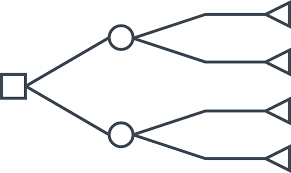
\includegraphics[height=0.3\textheight]{capitulo2/images/arbol-decision-ejemplo.png}
		\caption{Representación general de un árbol de decisión}
		\label{fig:arbol-decision-ejemplo}
	\end{center}
\end{figure}

\subsection{ID3 (Iterative Dichotomiser 3)} \label{id3}

El algoritmo ID3 es uno de los algoritmos que utilizan árboles de decisión más populares. ID3 genera un árbol a partir de un conjunto de datos llamado \textbf{tabla de inducción}. Es útil para hacer toma de decisiones en escenarios binarios, es decir, que tienen 2 posibilidades finales.\\

El resultado de la ejecución de este algoritmo puede expresarse como un conjunto de reglas \textbf{\textit{si-entonces}}.

\subsubsection{Entropía}
La entropía es la medida de la aleatoriedad. En otras palabras, la medidad e la impredictibilidad. La entropía es más alta cuando todos los eventos posibles en un escenario son igualmente probables, por ejemplo, al tirar una moneda al aire, se tiene 50\% de probabilidad de que caiga cara y 50\% de probabilidad de que caiga cruz, por lo que la entropía es de 1. Este parámetro comienca a decrecer cuando hay una probabilidad o probabilidades que parezcan aplastantes sobre las otras. La fórmula para calcular la entropía es la siguiente:

\subsection{C4.5} \label{c4.5}

\subsection{Spark}
Es una herramienta de código abierto. Es un motor de análisis de datos unificado para Big Data y Machine Learning. 
\subsection{Hadoop}
Es un framework de software que soporta aplicaciones distribuidas bajo una licencia libre. Permite a las aplicaciones trabajar con miles de nodos y petabytes de datos. Hadoop se inspiró en los documentos Google para MapReduce y Google File System (GFS). Hadoop utiliza su propio sistema de archivos HDFS, que divide archivos grandes y los distribuye en diferentes nodos para su procesamiento.

\begin{enumerate}
	\item Solicite administrar los pagos admisión seleccionando la opción \textbf{Administración de pagos} del menú \refIU{fig:menuPrincipalCG}{Menú del Contador General} y posteriormente la opción \textbf{Pagos Admisión} del menú \refIU{fig:menuPagosA}{Menú Pagos Admisión}.
	\item Se mostrará la pantalla \refIU{fig:ss}{Administrar Pagos Admisión}.
	\begin{figure}[!htbp]
		\hypertarget{fig:ss}{\hspace{1pt}}
		\begin{center}
			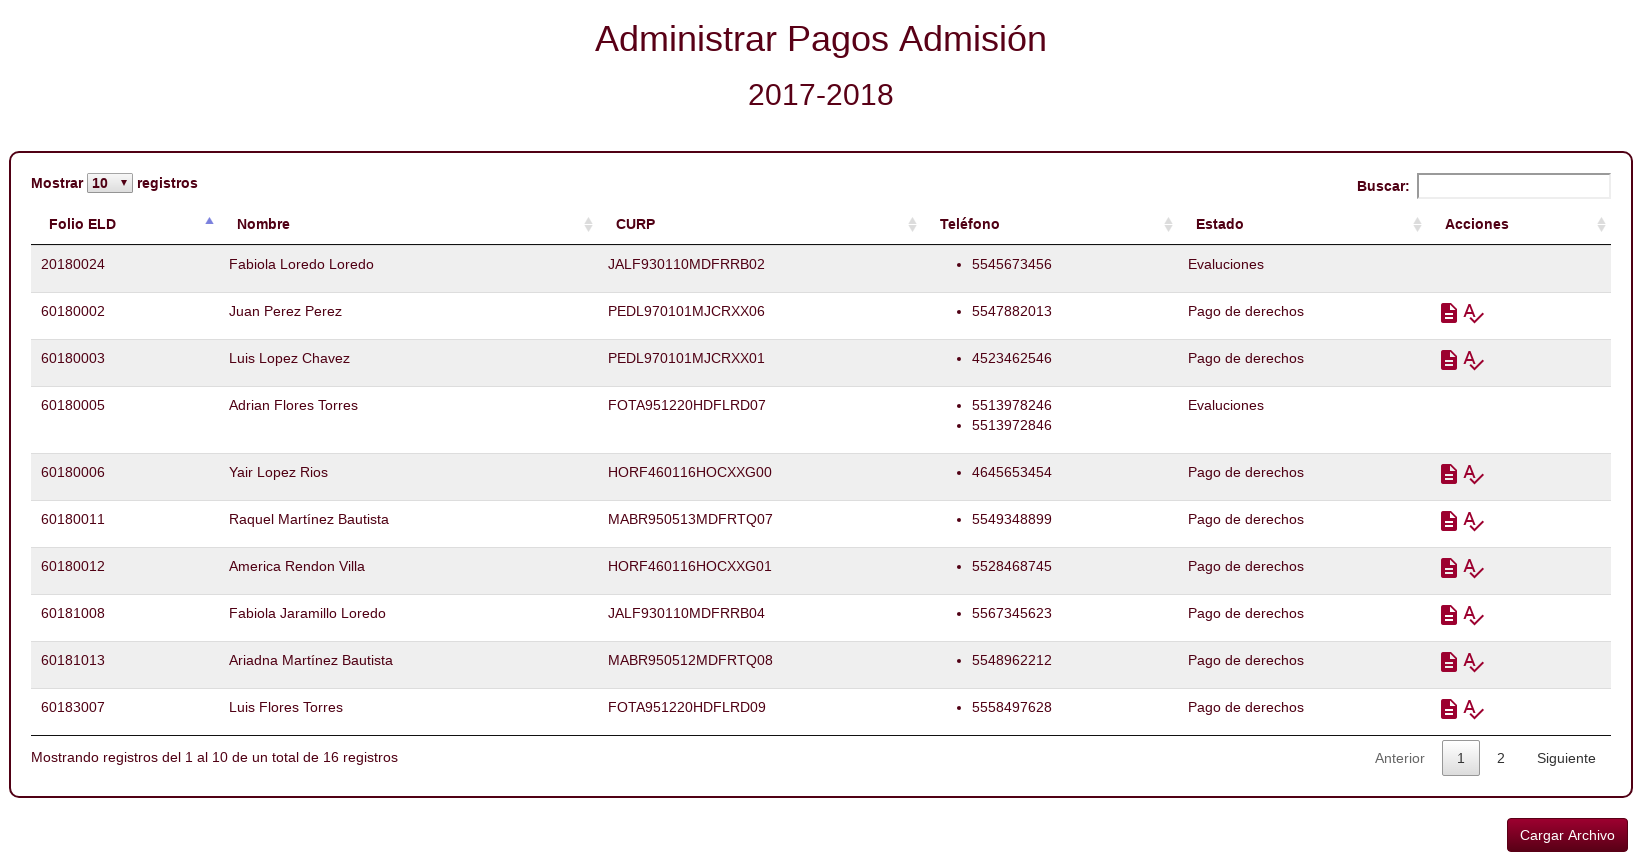
\includegraphics[height=0.3\textheight]{capitulo1/images/IU-APA.png}
			\caption{Administrar Pagos Admisión}
			\label{fig:ss}
		\end{center}
	\end{figure}

	
\end{enumerate}

\newpage
\begin{Errores}
	\error{El sistema muestra un mensaje indicando que falta información para realizar la operación.}
	{
		\begin{UClist}
			\UCli	Verifique que exista una convocatoria \textbf{Publicada}.
			\UCli	Verifique que exista un periodo de pagos.
			\UCli	Verifique que exista un periodo de pre-registro CENEVAL vigente.
		\end{UClist}
	}
	\error{El sistema muestra un mensaje indicando que no se ha realizado la asociación de fechas de CENEVAL y Psicométrico.}
	{
		\begin{UClist}
			\UCli	Verifique que la Coordinación de Control Escolar haya asociado las fechas CENEVAL y Psicométrico.
		\end{UClist}
	}
	

\end{Errores}
